\section{Task 1}

% LINK https://towardsdatascience.com/ways-to-detect-and-remove-the-outliers-404d16608dba
\subsection{Edge Weight Selection}\label{sec:weights}
The edge-weights were selected using information from  both datasets \DSone{} and \DStwo{}; after selection  these weights are then normalized in order to better be exploited by the linear threshold model. The formula used to compute these edge weights, prior the normalization step, is quite intuitive and can be described as the sum of the number of articles containing the both keywords $k_1$ and $k_2$, weighted by the rank of the articles' authors. The rank is obtained by computing the \textit{pagerank} of the author graph of the respective year.\\
The formulation of these pre-normalization edge weights (for example, between keywords $k_1$ and $k_2$) is given by
\begin{equation}\label{eq:weight_prenorm}
w_{k_1,k_2}=\sum_{a_i} \mathrm{rank}(a_i)\cdot \mathrm{count}_{k_1,k_2}(a_i)    
\end{equation}
where $a_i$ varies over the set of all authors, ${rank}(a)$ is the pagerank of author $a$, and ${count}_{k_1, k_2}(a)$ is the number of articles having as author $a$ and containing both $k_1$ and $k_2$.
The pagerank of an author (for a given year $y$) is obtained by computing the pagerank of co-authorship graph for the respective year.

% TODO add outlier detection
\paragraph{\textbf{Outlier Correction.}} One problem that was encountered during the first phase of the project was the presence of outlier edge-weights. Indeed, the weights computed using the \cref{eq:weight_prenorm} can be heavily unbalanced (as can be seen in  \cref{fig:weight_prenorm}), which caused a number of problems when trying to apply the linear threshold algorithm. This problem was approached by using a simple outlier correction strategy; using the \textit{z-score} of the edge-weight distribution, clamping elements with a \textit{z-score} higher than three.

  \begin{figure}[h!]
     \centering
     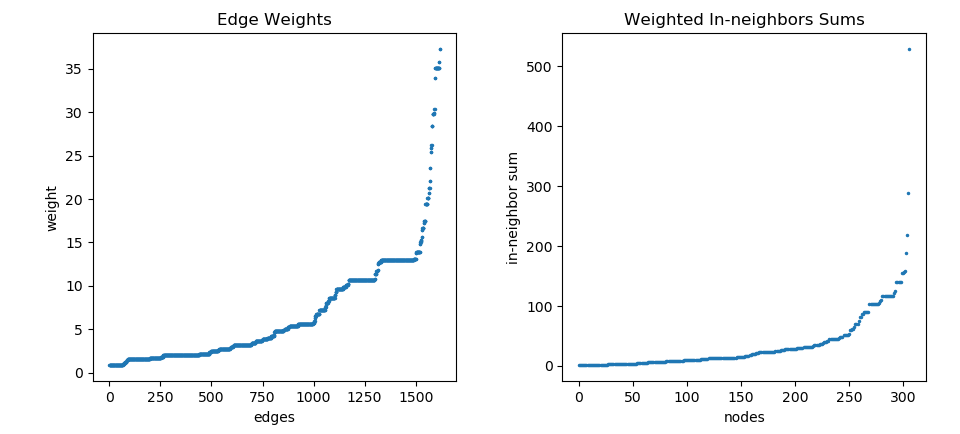
\includegraphics[width=\textwidth]{img/prenorm.png}
     \caption{Graphs showing the distribution of the edge-weights and of the in-neighbors sums \textbf{before} the normalization step.}
     \label{fig:weight_prenorm}
 \end{figure}
 
\paragraph{\textbf{Normalization.}}
As previously mentioned, in order to use these calculated edge-weights with the linear threshold algorithm (see \cref{sec:ltm}), a normalization step is necessary. 
 Indeed, remember that the in-neighbors sums must be less then or equal to one for each node in the input graph, which may not be true for the weights computed using \cref{eq:weight_prenorm}. Another problem is that if the in-coming weights of a node are too small then they will not be able infect it, hence blocking the diffusion process.\\ 
 A number of possible strategies can be used in order to avoid these situation, in particular, for this project three types were considered:
 \begin{itemize}
     \item The simplest normalization strategy is to scale all the weights $w_{u,v}$ such that  \cref{eq:linear_threshold_constraint} must be valid for all nodes $u$. This can be achieved by dividing all the weights by the maximum in-neighbors sum. That is,
     \[\hat w_{v,u} = \frac{w_{v,u}}{\displaystyle \vphantom{\bigg(} \max_{y} \Big\{\sum_{x\in \InNeighbours(y)} w_{x,y}\Big\}}\]
     This normalization, however, caused the edges' weights to be far too unbalanced, favouring nodes with a high number of in-neighbours, and virtually never activating nodes with fewer incoming edges.
     \item Another strategy initially adopted consisted in forcing the sum of all the in-coming neighbors of all nodes to be $1$. This can be accomplished by locally scaling each weight with the formula
     \[
     \hat w_{v,u} =\frac{w_{v,u}}{\displaystyle \sum_{v'\in \InNeighbours(u)}w_{v',u}}
     \]
     The major drawback of this approach is that nodes with a single incoming vertex  are always activated with their incoming neighbor. More generally, nodes with a low number of in-coming neighbours are favoured while using this normalization approach.
     \item The final normalization strategy, which is the one actually adopted in this project, consists in employing a logarithmic balancing of the in-neighbors summations.
     \[
     \hat w_{v,u} = \frac{w_{v,u}}{\vphantom{\bigg(} \displaystyle \log\Big( 1 + \sum_{x\in \InNeighbours(u)}w_{x,u}\Big)}\cdot z
     \]
     with $z$ a normalization factor such that 
     \[\max_{u}\Big\{ \sum_{v\in \InNeighbours{u}}\hat w_{v,u} \Big\} = 1\]
     The use of the logarithm allows the in-neighbors sums to be well distributed, so that nodes with less nodes can be activated. This method proved to create topics that are somewhat balanced. It is possible to see the difference between before and after this normalization process respectively in \cref{fig:weight_prenorm} and \cref{fig:weight_afternorm}.
 \end{itemize}
 
\begin{figure}[h!]
     \centering
     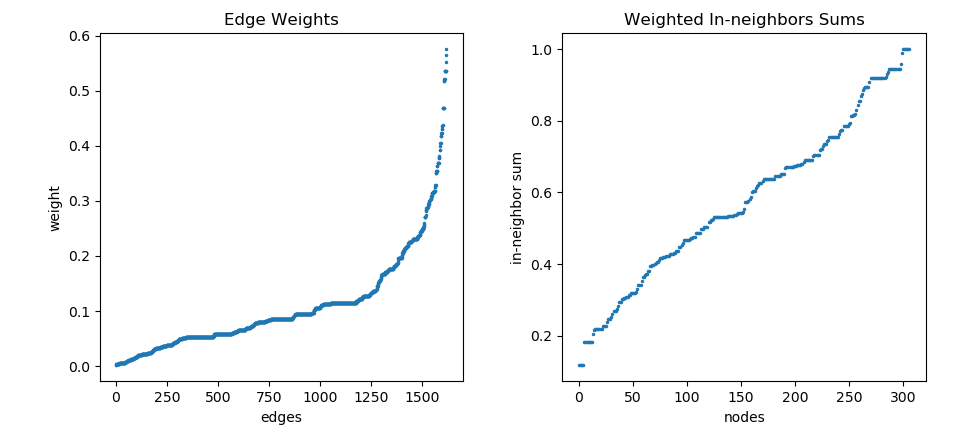
\includegraphics[width=\textwidth]{img/afternorm.png}
  \caption{Graphs showing the distribution of the edge-weights and of the in-neighbors sums \textbf{after} the normalization step.}
  \label{fig:weight_afternorm}
 \end{figure}
  

 
\subsection{Topicness}\label{subsec:topicness}
Following the project's specification, topics are estimated by applying the linear threshold model over some source nodes, which have to be extracted using a metric to define, \ie{} pagerank, cluster-coefficient, \etc{}. During development, different such metrics were tested and refined. At first, the pagerank was utilized in order to pick the best candidates. However, two major problems resulted from using pagerank: a strong bias towards hubs (which are not necessarily good topic sources), and a problem with the \enquote{picking} strategy, since simply taking the nodes with highest value will take nodes most likely near to the core of the graph's main component.\\
To solve the first problem a combination of metrics were utilized, specifically, two others besides pagerank: \textit{Local Cluster Coefficient}, and \textit{Betweenness Centrality}. The local cluster coefficient of a node indicates how much the neighbors of a node are interconnected with each-others; it is intuitive that good topics sources have an higher cluster coefficient than normal nodes. For un-directed un-weighted graphs, the cluster coefficient of $u$ is described by
\[
\mathrm{cluster\ coefficient}(u) = \frac{2\Big|\Big\{\{v,w\}\in \Edges:v\in\Neighbours(u), w\in\Neighbours(u)\Big\}\Big|}{d_u\cdot(d_u - 1)}
\]
However, the directed weighted variant described in \cite{clustering} (implemented by \textbf{NetworkX}) was used for this project.

It was possible to improve the initial pagerank estimation by adding the information found in the cluster coefficient. This was done by using, instead of standard pagerank, the \textit{personalized-pagerank} algorithm, with personalization vector the cluster-coefficient (after being appropriately scaled to a probability distribution).
The difference, using as dumping factor $0.8$, can be seen in \cref{fig:pagerank_comparison}.
\begin{figure}[h!]
		\centering
		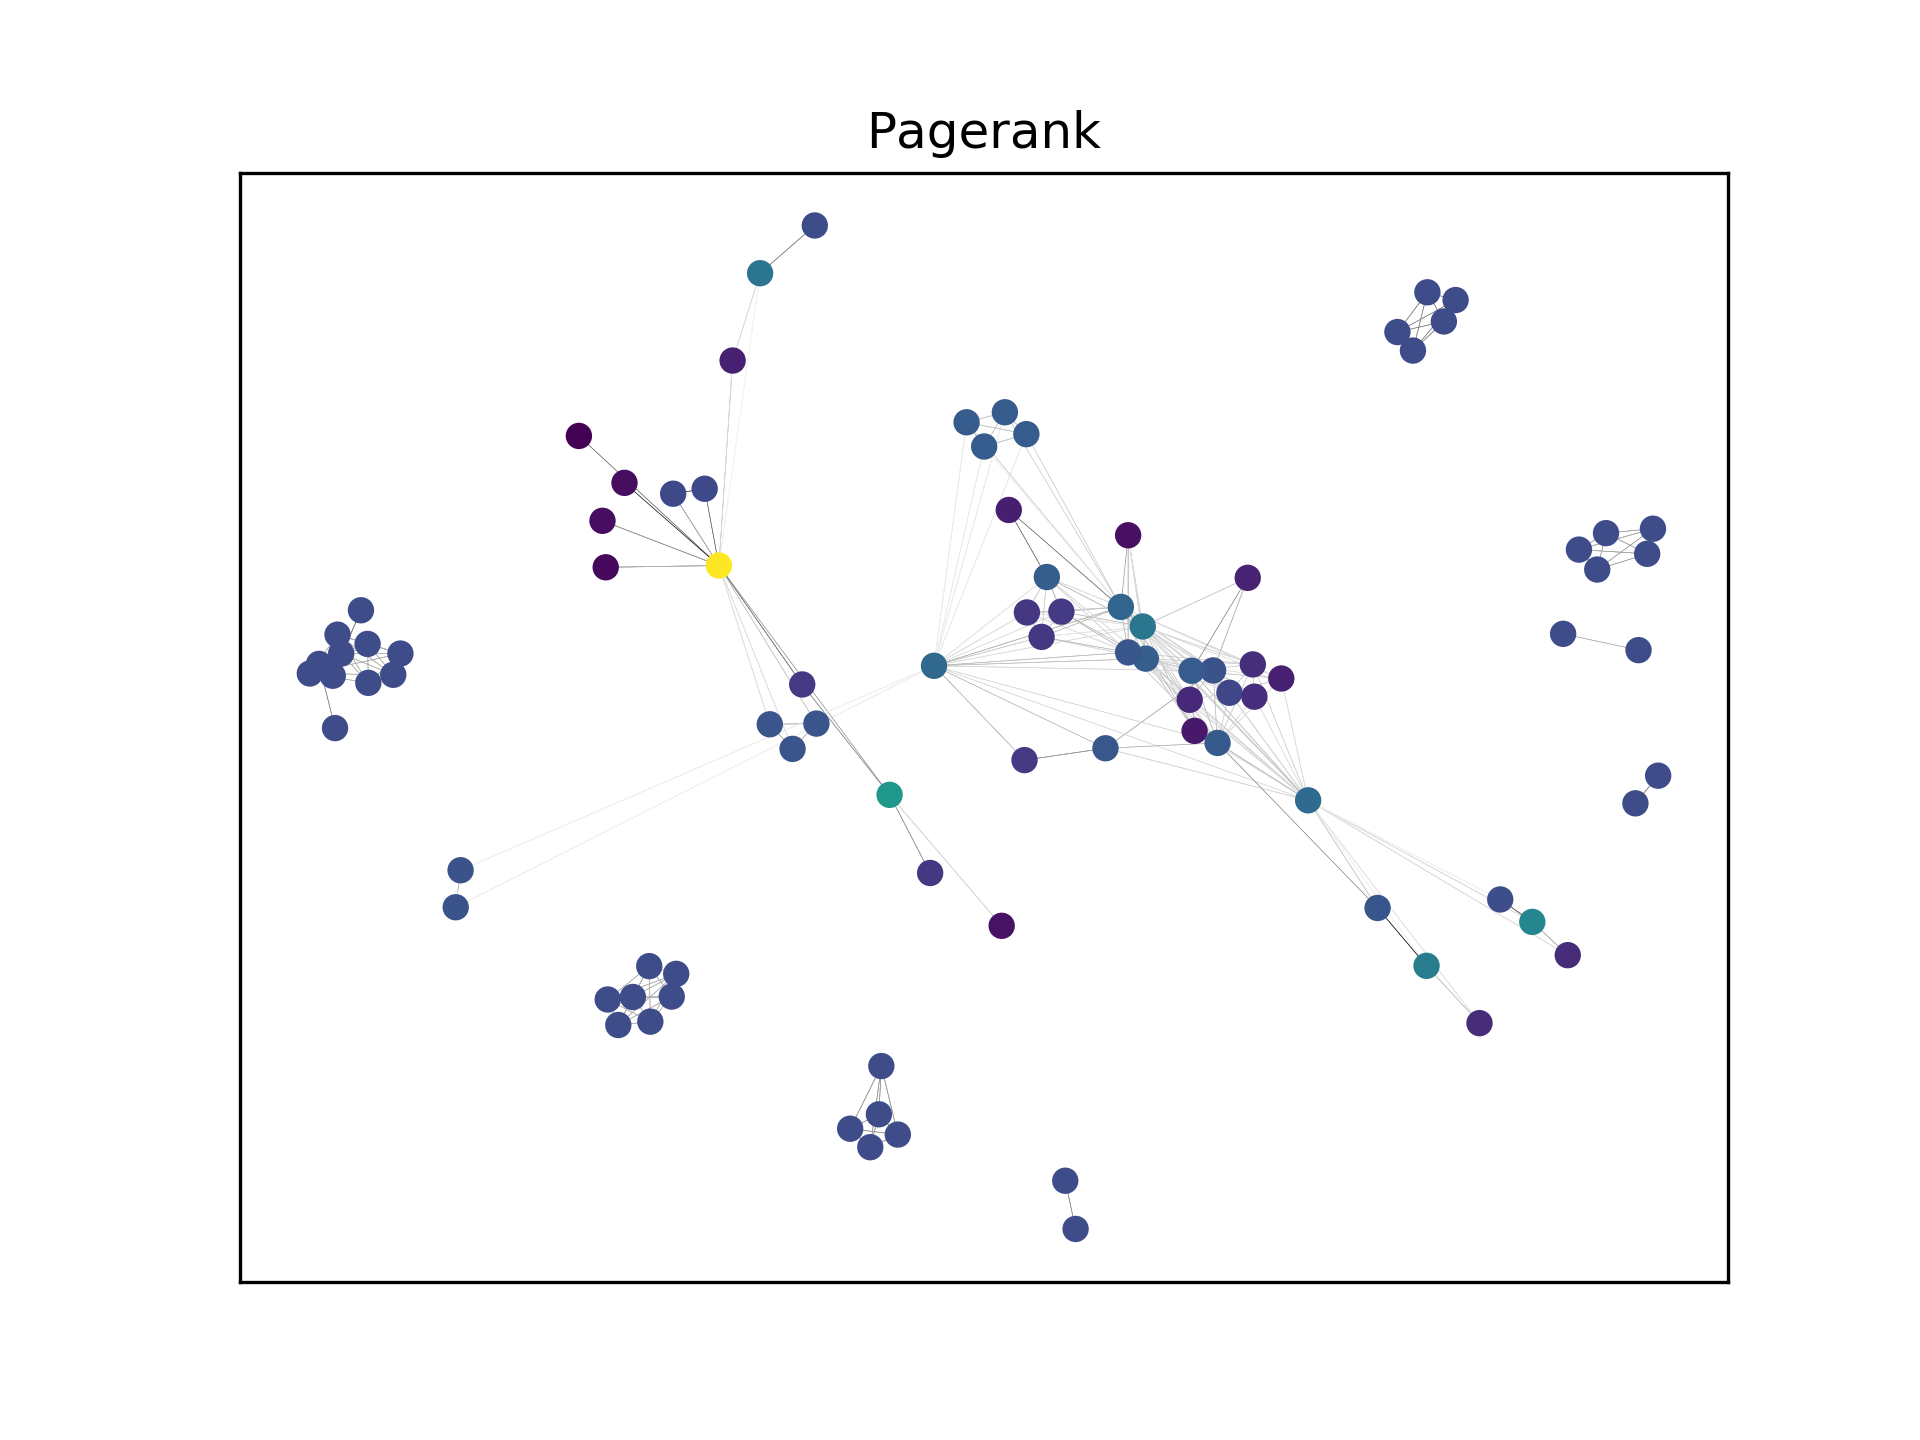
\includegraphics[width=.495\textwidth]{img/pr.png}
		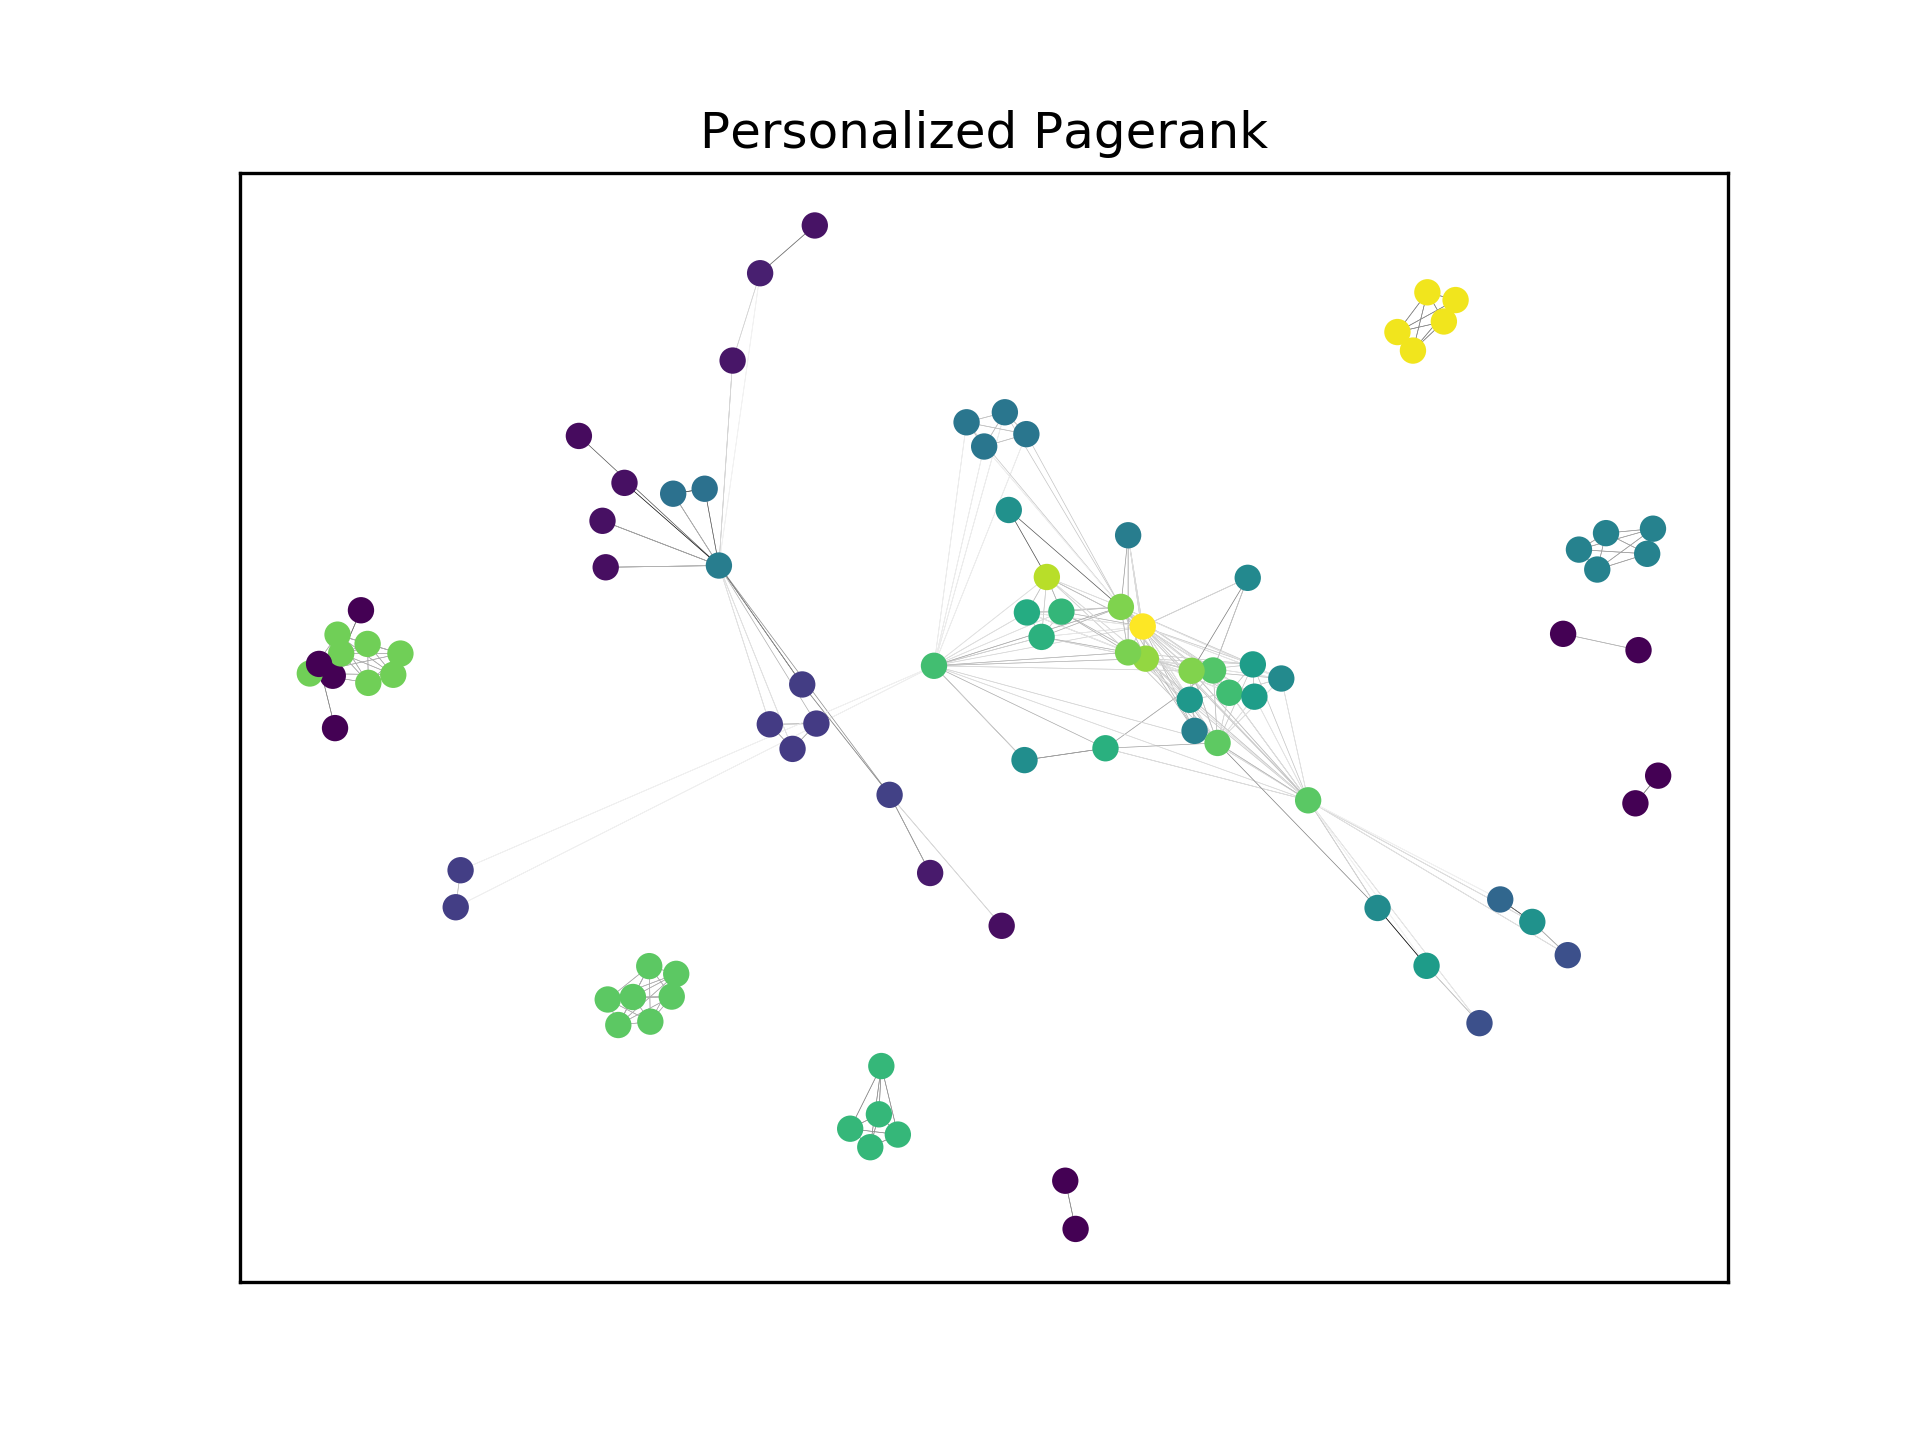
\includegraphics[width=.495\textwidth]{img/ppr.png}\\
		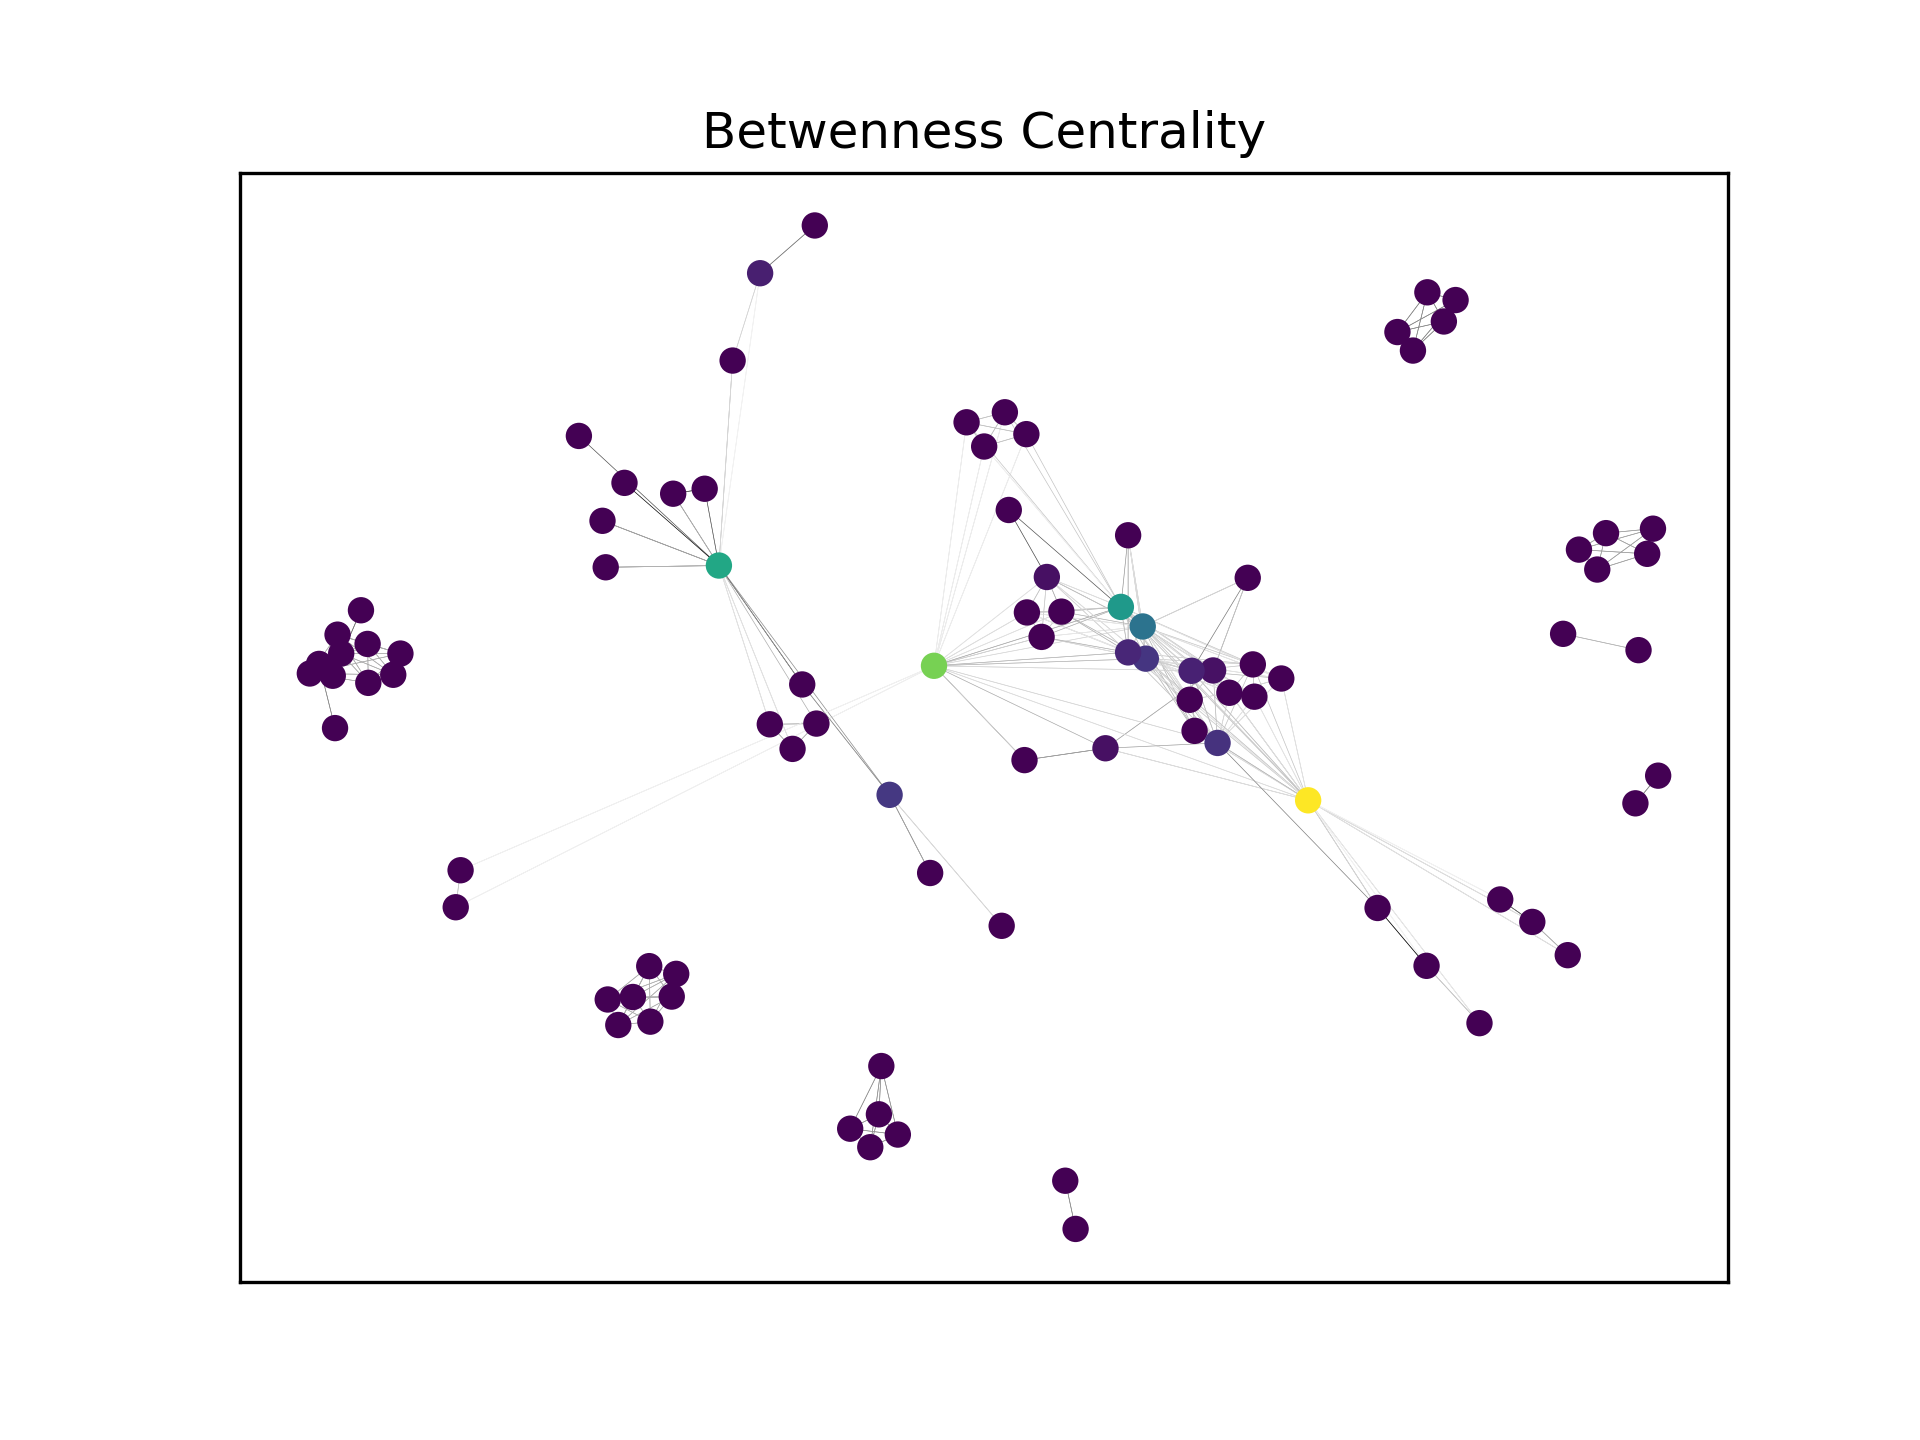
\includegraphics[width=.495\textwidth]{img/bc.png}
		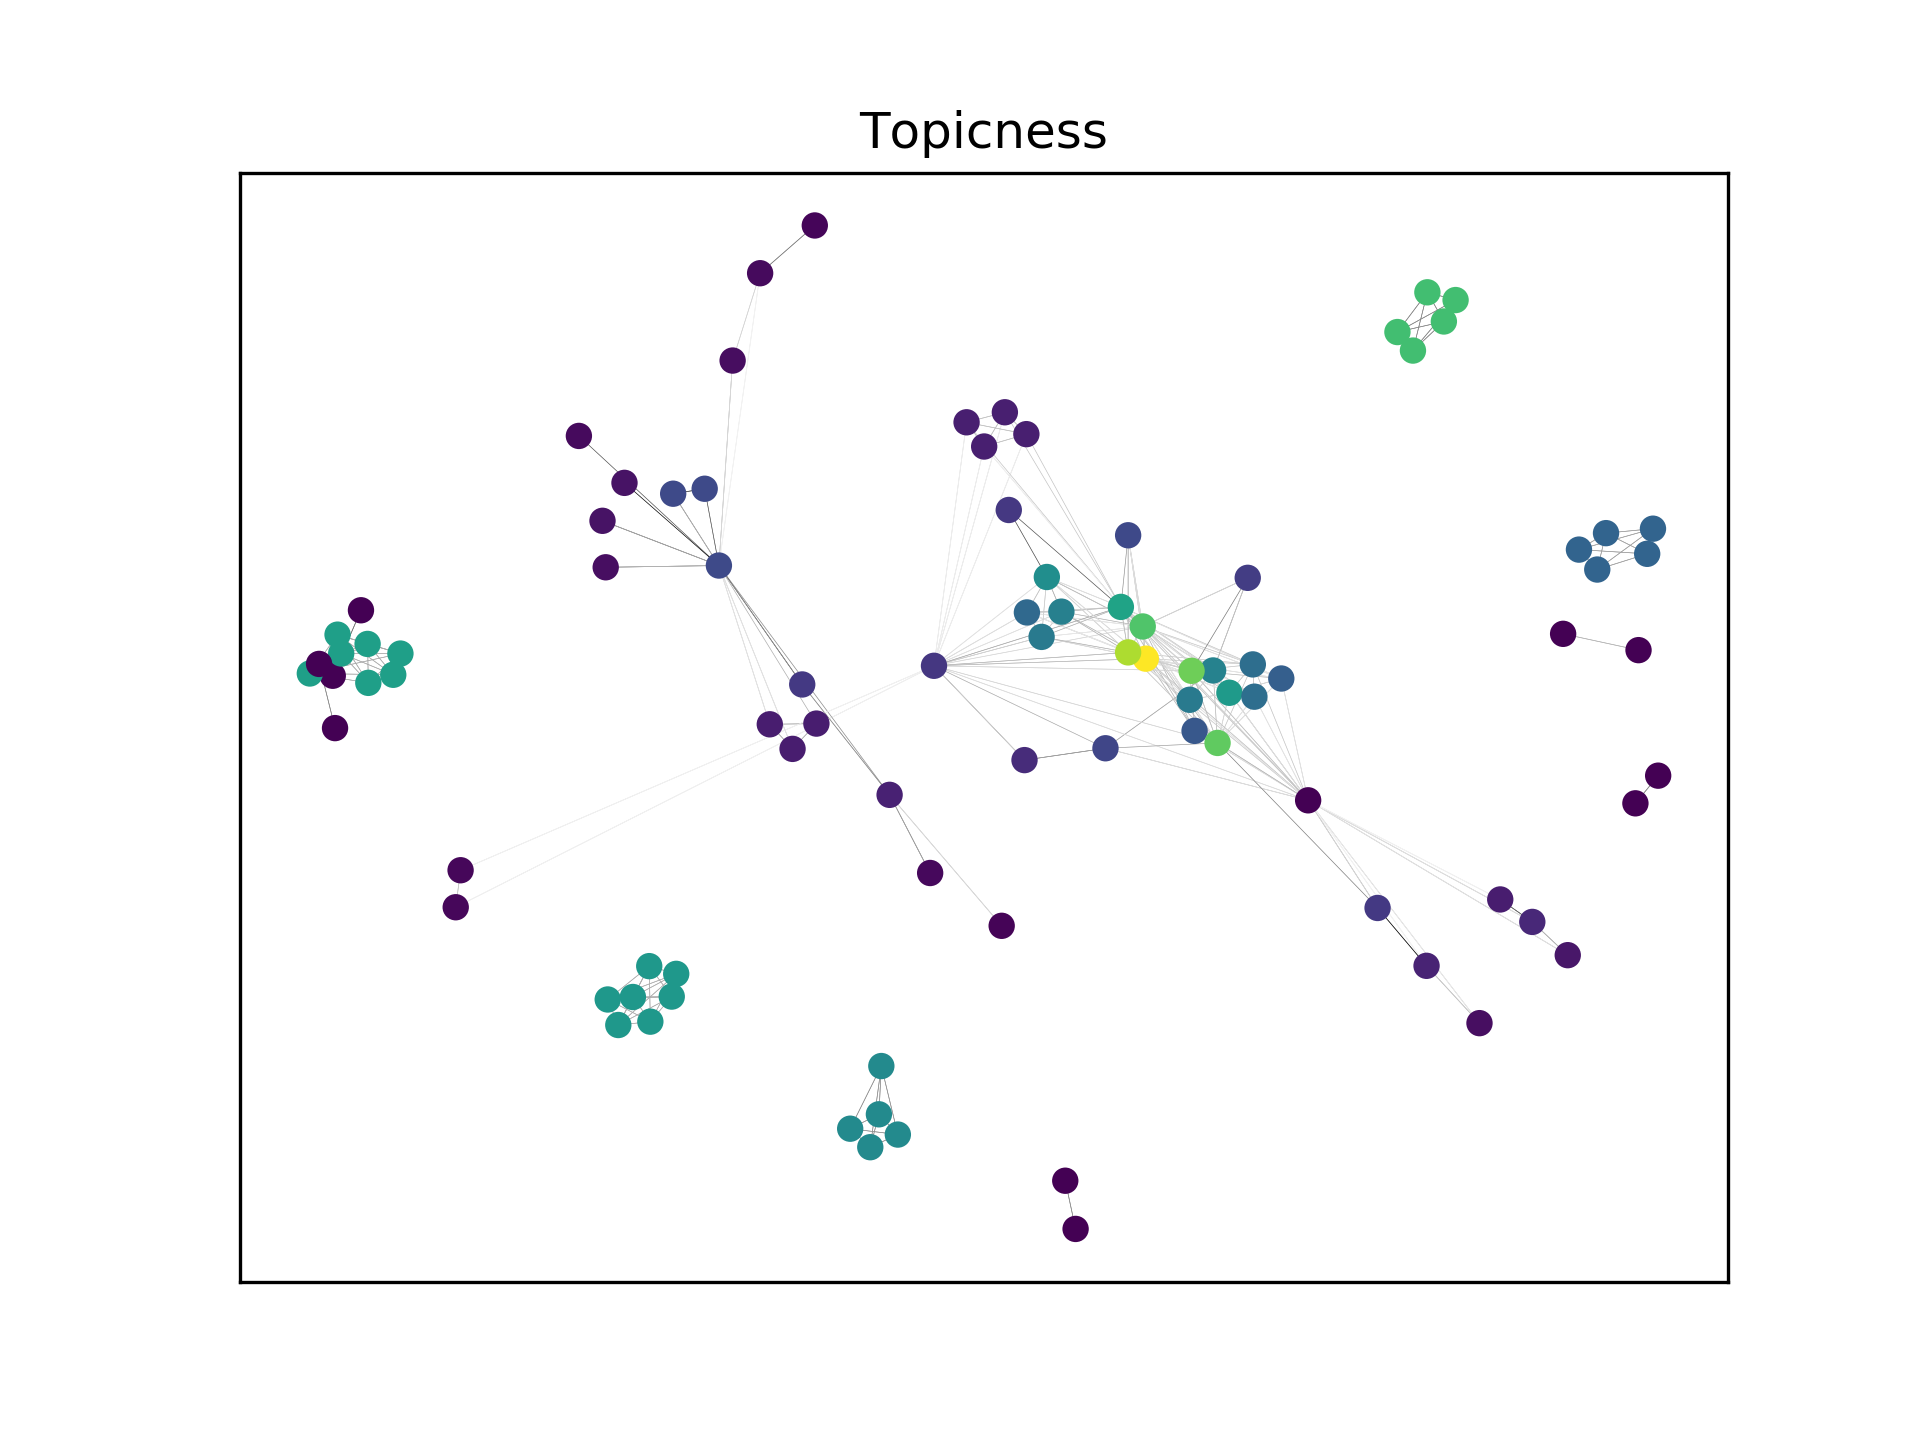
\includegraphics[width=.495\textwidth]{img/tp.png}
		\caption{Comparison between standard Pagerank, Personalized Pagerank (using local Cluster-Coefficient), Betwenness Centrality, and Topicness.}
		\label{fig:pagerank_comparison}
\end{figure}
Despite improving on the initial function, the personalized-pagerank remained yet too inclined towards really big hubs; in order to reduce this bias a new metric was introduced, the aforementioned betweenness centrality. The personalized pagerank values are scaled down proportionally to their betweenness score, which was found to be impacting only nodes that represents big \enquote{hubs} in the graph. The resulting metric, denoted as \textit{topicness}, is hence given by the equation:  
\begin{equation}\label{eq:topicness}
\mathrm{topicness}(u) = \mathrm{personalized\text{-}pagerank}(u)\cdot \Big(1-\mathrm{betweenness}(u)\Big) 
\end{equation}
for each $u\in \Vertices$. 

\subsection{Topic Extraction} Topics are extracted using an iterative method: at each iteration the node associated to the global maximum value\footnote{If there is more then one maximum, then the node is arbitrarily chosen  between those.} of the topicness function is  extracted; after that, the influence of said node is used to update the topicness "surface", in order to obtain a different maximum in the next iteration (see \cref{alg:topic_extraction}).
\newcommand{\Topicness}{\mathop{\texttt{topicness}}}
\begin{algorithm}[H]
\caption{Topic Extraction}\label{alg:topic_extraction}
\begin{algorithmic}[1]
    \Require{$\mathrm{graph}$, keyword co-occurrence graph for a specific year, with $n$ vertices.}
    \Require{$\Topicness$, array of size $n$, indicating topicness for each node.}

    \Statex
    \Procedure{topic\textunderscore{}extraction}{$\mathrm{graph}$, $\Topicness$}
    \State{$S\leftarrow \emptyset$}
	\While{$\exists x: \Topicness[x] > 0$}
	   \State $\mathrm{maxnode} \leftarrow \mathrm{argmax}_{v}\{\mathrm{topicness}[v]\}$ 
	   \State $\mathrm{topic} \leftarrow \texttt{\color{AlgProcedureColor}node\textunderscore{}influence}(\mathrm{graph}, \mathrm{maxnode})$\Comment{$topic$ is an indicator array.}
	   \For{$u= 1 \dots n$}
	    \State $\Topicness[u] \leftarrow \Topicness[u]\cdot(1 - \mathrm{topic}[u])$
	   \EndFor
	   \State{$S\leftarrow S\cup \{\mathrm{maxnode}\}$}
	\EndWhile
    \State{\Return{S}}
	\EndProcedure
\end{algorithmic}
\end{algorithm}
\paragraph{\textbf{Node influence.}} The \texttt{\color{AlgProcedureColor}node\textunderscore{}influence} is computed using the average linear threshold algorithm, as described in \cref{sec:altm}; hence the variable $\mathrm{topic}$ is a vector of size $n$ with values between $0$ and $1$, indicating how much a certain node belongs to the topic identified by the chosen source node. During the project development two methodologies were tested for choosing the value of the topic vector:
\begin{description}
\item[Fuzzy:] At first, the topics were considered as fuzzy topics, using the output of the average linear threshold as description of the topic.
However, this caused some problems during the tracking phase, as topics tended to be too unbalanced towards the source (whose membership value is always one).
\item[Crisp:] After the problems induced by the fuzzy sets during the second task, it was decided to use standard (\ie{} crispy) sets in order to describe topics. Of course, this requires a \textit{defuzzification} procedure, which may loose information.
\end{description}



\subsection{Defuzzification of topics}
Fuzzy set theory uses several strategies in order to converted fuzzy sets to standard sets. These may range from mean based techniques, to more sophisticated algorithms. In our case, the algorithm is fairly simple; the $k=6$ nodes with higher membership values (only if they are different from zero) are considered as the crisp representation of the topic. More formally, if $x$ is in the defuzzification $S$ of $\Fuzzy{F}$, then 
$$
    x\in S \implies \begin{cases}
    \forall y\not\in S: \mu_{\Fuzzy{F}}(x) \ge \mu_{\Fuzzy{F}}(y)\\
    \mu_{\Fuzzy{F}}(x) > 0
    \end{cases}
$$
and the size of $S$ must be less then or equal to $k$ (\ie{} $|S| \le k$).
This is done in order to prevent the creation of topics  that are either too big or too small, and six was experimentally a good number for topic size. The conversion procedure can be seen in \cref{alg:defuzzification}.
\begin{algorithm}
\caption{Defuzzification}\label{alg:defuzzification}
\begin{algorithmic}[1]
    \Require{$F$, sequence of length $n$ and containing pairs $(x,\mu_{\Fuzzy{F}}(x))$. This object represents the fuzzy set $\Fuzzy{F}$}
    \Statex
    \Procedure{defuzzification}{$F$, $k$}
        \State{} $ S \leftarrow \emptyset$ 
        \State{} Sort array $F$ w.r.t. membership values.
        \For{$i= n-k \dots n$}
        \State{} $(x,\mu_{\Fuzzy{F}}(x))\leftarrow F[i]$
        \If{$\mu_{\Fuzzy{F}}(x) > 0$}
         $S\leftarrow S \cup \{x\}$
        \EndIf
	\EndFor
	\State \Return{S}
	\EndProcedure
\end{algorithmic}
\end{algorithm}



